\documentclass{standalone}
\usepackage{ tikz }
\usepackage{ xparse }
\usepackage{ ../../../macros }

\begin{document}
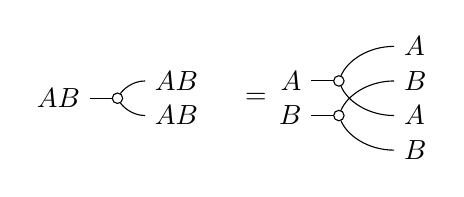
\begin{tikzpicture}[yscale=-1,x=1em,y=1.25em]
    \node [anchor=east] at (-1,0) {$A \tensor B$};
    \draw [] (-1,0) -- (0,0);
    \node (C1) [draw, circle, fill=white, scale=0.4] at (0,0) {};

    \node (A1) [anchor=west] at (1,-0.5) {$A \tensor B$};
    \node (A2) [anchor=west] at (1,0.5) {$A \tensor B$};

    \draw (C1) to[out=285, in=180] (A1);
    \draw (C1) to[out=75, in=180] (A2);

    \node at (5,0) {$=$};

    \node [anchor=east] at (7,-0.5) {$A$};
    \node [anchor=east] at (7,0.5) {$B$};

    \draw (7,-0.5) -- (8,-0.5);
    \draw (7,0.5) -- (8,0.5);

    \node (C2) [draw, circle, fill=white, scale=0.4] at (8,-0.5) {};
    \node (C3) [draw, circle, fill=white, scale=0.4] at (8,0.5) {};

    \node (A3) [anchor=west] at (10,-1.5) {$A$};
    \node (A4) [anchor=west] at (10,-0.5) {$B$};
    \node (A5) [anchor=west] at (10,0.5) {$A$};
    \node (A6) [anchor=west] at (10,1.5) {$B$};

    \draw (C2) to[out=285, in=180] (A3);
    \draw (C2) to[out=75, in=180] (A5);
    \draw (C3) to[out=285, in=180] (A4);
    \draw (C3) to[out=75, in=180] (A6);

\end{tikzpicture}
\end{document}